\documentclass{beamer}
\usepackage[utf8]{inputenc}
\usepackage{xeCJK} 
\usepackage[T1]{fontenc}
\usepackage{mathabx}
\usepackage{amsmath} 
\usepackage{mathpazo}
\usepackage{bibentry}
\usepackage{tikz}
\usepackage{caption}
\usepackage{graphicx, subfig}

\usetikzlibrary{scopes}
\def\iangle{35} % Angle of the inclined plane
\def\down{-90}
\def\arcr{0.5cm} % Radius of the arc used to indicate angles

\usetheme{Boadilla}
\usecolortheme{wolverine}
\useoutertheme{miniframes}

\title{VP160 Midterm Review Class}
% \subtitle{Non-inertial FoR}
\author{Zeyi Ren}
\institute{UM-SJTU Joint Institute}

\begin{document}

\maketitle

\begin{frame}
  \begin{enumerate}[1.]
    \item Scientific Notations
    \begin{itemize}
      \item $ a\times 10^n$ ($1\leq |a| < 10$)
      \item Usually used for very large number or very small number like computation in Astrophysics or Quantum Mechanics.
      % \item e.g.\\Gravitation constant $G = 6.67384\times 10^{-11} N\cdot m^2\cdot kg^{-2}$\\ Planck constant $h = 6.62606896\times 10^{-34} J\cdot s$
    \end{itemize}\pause
    \item Unit Prefix and Conversion
    \begin{itemize}
      \item \textcolor{red}{$k$} (unit prefix) \textcolor{blue}{$m$} (unit)
      \item Some commonly-used unit prefixes:\\ 
      \begin{table}[H]
        \begin{tabular}{c|c|c|c|c|c|c|c}
        \hline
        $p$        & $n$       & $\mu$     & $m$       & $c$       & $k$      & $M$      & $G$      \\ \hline
        $10^{-12}$ & $10^{-9}$ & $10^{-6}$ & $10^{-3}$ & $10^{-2}$ & $10^{3}$ & $10^{6}$ & $10^{9}$ \\ \hline
        \end{tabular}
        \end{table}
        
        CASIO fx-991CN X $\rhd$ $\boxed{OPTN}$ $\rhd$ $3:$工程符号\\
        e.g.\\Input: 1m; Output: $\frac{1}{1000}$
    \end{itemize}\pause
    \item Basic Units \& Derived Units
    \begin{itemize}
      \item SI system of units: 
      \begin{table}[H]
        \begin{tabular}{c|c|c|c|c|c|c|c}
        \hline
        Quantity & $L$        & $m$       & $t$       & $I$       & $T$       & $n$      & $lv$     \\ \hline
        Unit     & \textcolor{black}{$m$} & $kg$& $s$ & $A$ & $K$ & $mol$ & $cd$ \\ \hline
        \end{tabular}
        \end{table}
    \end{itemize}
  \end{enumerate}
\end{frame}

\begin{frame}{Dimensional Analysis: System of Units}
  % \begin{block}{Dimensional Analysis: System of Units}
\begin{enumerate}
  \item We can first select some physical quantities as the ``\textbf{basic quantities}”
  and specify a ``\textbf{unit for measurement}” for each basic quantity,
  the other physical quantities' units can be derived from the
  relation between them and the fundamental
  quantities. These physical quantities are called \textbf{derived quantities}
  and their units It's called \textbf{derived unit}.\pause
  \item A set of units derived in this way, is called a \textbf{system of units}.\pause
  \item We often use capital letter to represent a ``dimensional quantity", and
  use [$x$] to represent the ``dimensional quantity" of specific physical quantity $x$.\\
  e.g. The dimensional quantity of a particle of mass $m$ is written as: $M$ = [$m$].
\end{enumerate}
% \end{block}
\end{frame}

\begin{frame}{Dimensional Analysis: Method of Undetermined Coefficients}
\textcolor{blue}{Exercise 1}

A simple pendulum consists of a light inextensible string AB with length $l$, with the end $A$ fixed, and a point mass $m$ attached to $B$. The pendulum oscillates with a small amplitude, and the period of oscillation is $T$. It is suggested that $T$ is proportional to the product of powers of $m$, $l$ and $g$, where $g$ is the acceleration due to gravity. Use dimensional analysis to find this relationship.
\end{frame}

\begin{frame}{Back-of-the-envelop Problems}
  \begin{block}{Definition}
    A quick estimation of some physical quantities.
  \end{block}
  \begin{block}{Tips}
    \begin{enumerate}
      \item Try to remember the order of magnitude of some important constant.
      \item This type of questions may occur in exams.
    \end{enumerate}
  \end{block}
\end{frame}

\section{Vectors}
\begin{frame}{Basic Vector operations}
  \begin{itemize}
    \item Addition \& Subtraction\\ $$\vec{u}\pm \vec{v}=(u_1\pm v_1,u_2\pm v2,u_3\pm v_3)$$
    \item Scalar Multiplication$$\lambda \vec{u} = (\lambda u_1, \lambda u_2, \lambda u_3)$$
    \item Dot Product$$\vec{u}\cdot \vec{v} = |u||v|cos\theta=u_1v_1+u_2v_2+u_3v_3$$
    \item Orthogonal Projection Vector of the vector $\vec{u}$ onto the vector $\vec{v}$$$\frac{\vec{u}\cdot \vec{v}}{|\vec{v}|}\cdot \frac{\vec{v}}{|\vec{v}|}$$
  \end{itemize}
\end{frame}

\begin{frame}{Basic Vector operations}
  \begin{itemize}
    \item Cross Product
    \begin{itemize}
      \item Magnitude: $|\vec{u}\times \vec{v}|=|\vec{u}||\vec{v}|sin\theta$
      \item Direction: determined by \textbf{Right Hand Rule}
      \item Matrix expression(Using determinant):
      \begin{align*}
        \vec{u}\times \vec{v} &= \left|\begin{matrix}\hat{i}&\hat{j}&\hat{k}\\u_1 & u_2 & u_3\\ v_1 & v_2 & v_3 \end{matrix}\right|\\&=(u_2v_3-u_3v_2)\hat{i}+(u_3v_1-u_1v_3)\hat{j}+ (u_1v_2-u_2v_1)\hat{k}
 \end{align*}
    \end{itemize}\pause
    \item anti-commutative
    $$
    \vec{u}\times \vec{v} = -\vec{v}\times \vec{u}
    $$\pause
    \item Scalar Triple Product:$$\vec{u}\cdot(\vec{v}\times \vec{w})=\vec{v}\cdot(\vec{w}\times \vec{u})=\vec{w}\cdot(\vec{u}\times \vec{v})$$
  \end{itemize}
\end{frame}

\section{Kinematics}
\begin{frame}{1D Kinematics}
  \begin{itemize}
    \item Average vs. Instantaneous Quantities$$v_{x,A} = \frac{x(t+\Delta t)-x(t)}{\Delta t}\quad a_{x,A} = \frac{v(t+\Delta t)-v(t)}{\Delta t}$$
    \item Relationships\begin{align*}
    x &= x(t)\\
    v &= v(t)=\frac{d}{dt} x(t)\\
    a &= a(t)=\frac{d}{dt} v(t)=\frac{d^2}{dt^2}x(t)  
    \end{align*}
    \item Relative motion$$x = x_r + x';\quad v = v_r+v';\quad a=a_r+a'$$
  \end{itemize}
\end{frame}

\begin{frame}{Kinematics in 3D: Cylindrical Coordinates}
  \begin{block}{Basic Formulas in Cylindrical Coordinates}
    \begin{align*}\vec{r}&=\rho\hat{n_\rho}+z\hat{n_z}\\
  \vec{v}&=\dot{\rho}\hat{n_\rho}+\rho\dot{\phi}\hat{n_\phi}+\dot{z}\hat{n_z}\\
  \vec{a}&=(\ddot{\rho}-\rho\dot{\phi}^2)\hat{n_\rho}+(\rho\ddot{\phi}+2\dot{\rho}\dot{\phi})\hat{n_\phi}+\ddot{z}\hat{n_z}
  \end{align*}
\end{block}
  \textcolor{blue}{Tips:}\\
  if $z=0$, they become kinematics formulas in polar coordinates(see next slide).
\end{frame}

\begin{frame}{Kinematics in 2D: Polar Coordinates}
  \begin{block}{Basic Formulas in Polar Coordinates}
    \begin{align}\vec{r}&=r\hat{n_r}\\
      \vec{v}&=\dot{r}\hat{n_r}+r\dot{\theta}\hat{n_\theta}\\
      \vec{a}&=(\ddot{r}-r\dot{\theta}^2)\hat{n_r}+(r\ddot{\theta}+2\dot{r}\dot{\theta})\hat{n_\theta}
      \end{align}
  \end{block}\pause
  \begin{block}{Relations with cartesian coordinates}
    $$x=rcos\theta,\ y=rsin\theta$$
    $$d\vec{r}=dr\hat{n_r}+rd\theta\hat{n_\theta},\ |d\vec{r}|=\sqrt{(dr)^2+(rd\theta)^2}$$
  \end{block}
\end{frame}
%插入推导 withnotes 15 16

\begin{frame}{Kinematics in 3D: Natural Coordinates}
  \begin{block}{Basic Vectors}
    \begin{enumerate}
      \item $\hat{n_\tau}:$ along the direction of $\vec{v}$
      \item $\hat{n_n}$ and $\hat{n_b}$: perpendicular to the direction of $\vec{v}$
    \end{enumerate}
    $$
      \hat{n_\tau}=\frac{\vec{v}}{|\vec{v}|},\ 
      \hat{n_n}=\frac{\dot{\hat{n_\tau}}}{|\dot{\hat{n_\tau}}|},\ 
      \hat{n_b}=\hat{n_\tau}\times \hat{n_n}
      $$
  \end{block}\pause
  \begin{block}{Basic Formulas}
    $$\vec{v}=v\hat{n_\tau}$$
    $$\vec{a}=\dot{v}\hat{n_\tau}+\frac{v^2}{R_c}\hat{n_n}$$
    $R_c$ means radius of curvature, what is radius of curvature?
  \end{block}
\end{frame}
%插入19

\begin{frame}{Normal and Tangential, Radial and Transversal}
  \begin{figure}[htbp]
  \centering
  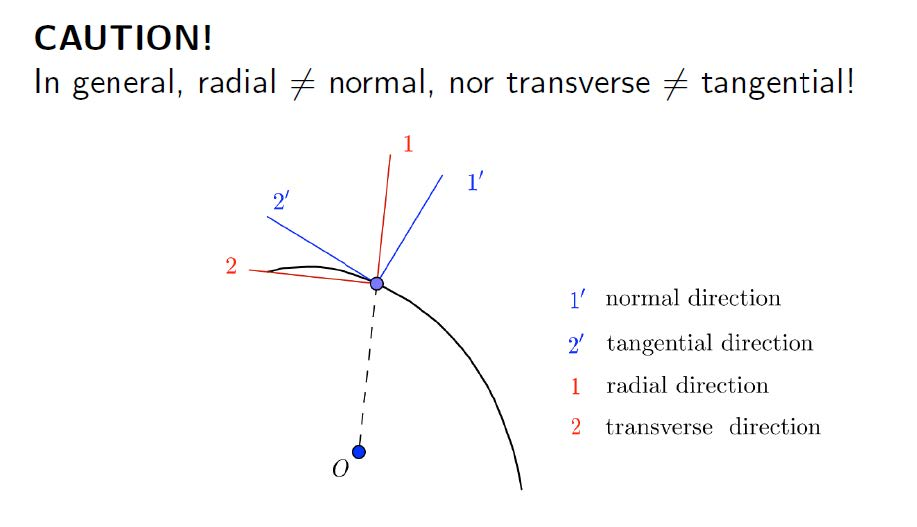
\includegraphics[width=1 \linewidth, angle =0]{Kinematics.png}
  % \caption{Difference between .}
  \label{fig:1}
  \end{figure}
\end{frame}

\begin{frame}{Useful Methods}
  \begin{enumerate}
    \item Separation of variables\pause
    \item Chain Rule
    $$a = \frac{dv}{dt}=\frac{dv}{dx}\cdot \frac{dv}{dt}=\frac{dv}{dx}\cdot v$$\pause
    \item Integral by parts:
    $$\int u'v = uv - \int v'u$$
  \end{enumerate}
\end{frame}
%example: t e^t
\begin{frame}
\textcolor{blue}{Exercise 2}

\begin{figure}[htbp]
\centering
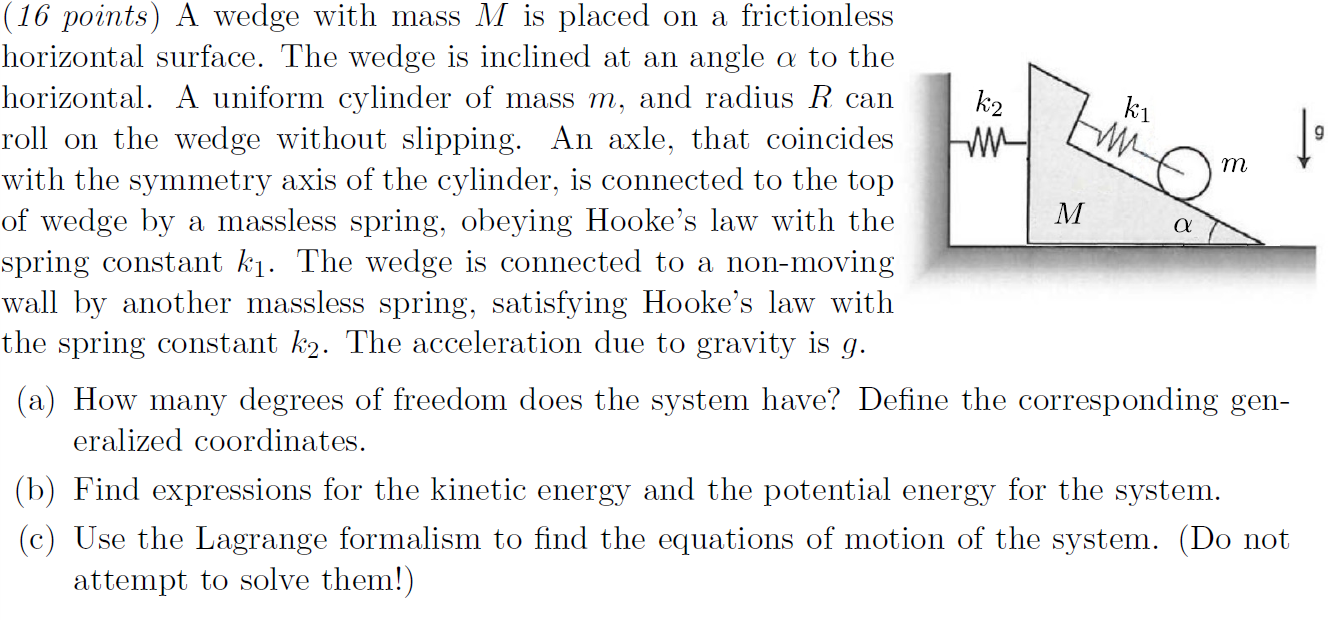
\includegraphics[width=1 \linewidth, angle =0]{ex1.png}
% \caption{.}
\label{fig:2}
\end{figure}
\end{frame}

\section{Force \& Inertial FoR}
\begin{frame}{Force and Inertial Frame of Reference}
  \begin{block}{Force}
    Force represents \textbf{interaction} between two objects or an object and its environment. 
  \end{block}\pause
  \begin{block}{Inertial frame of reference}
    In an inertial FoR, a physical object with zero net force acting on it moves with a constant velocity (which might be zero), or, equivalently, it is a frame of reference in which Newton's first law of motion holds.
 \end{block}
\end{frame}

\begin{frame}{Using Newton's Law in Complex System}
  \begin{enumerate}
    \item Objects at relatively rest $\rightarrow$ see as an whole.\pause
    \item Analyze forces between objects (relatively at rest or in motion) $\rightarrow$ isolate each of them.\pause
    \item To maintain a relatively static condition: $|f|\leq \mu_s N$\pause
    \item Use inertia force in Non-inertia FoR (usually objects with constant acceleration $\vec{a}$), $ \vec{F'} = m(-\vec{a})$.  
  \end{enumerate}
\end{frame}

\begin{frame}
\textcolor{blue}{Exercise 3}

\begin{figure}[htbp]
\centering
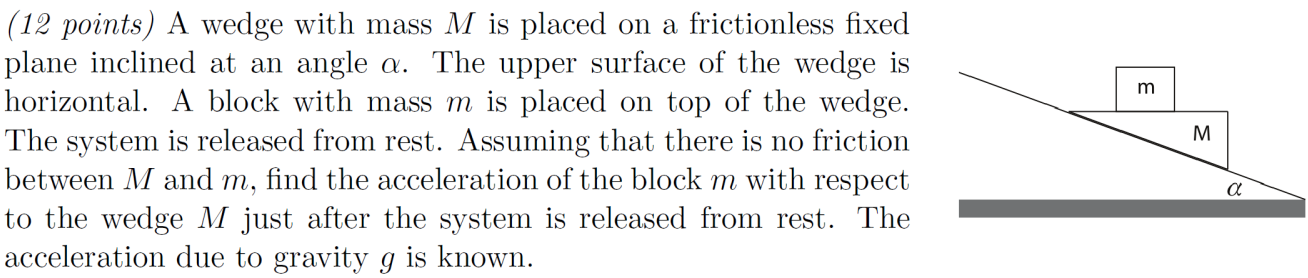
\includegraphics[width=1 \linewidth, angle =0]{ex3.png}
% \caption{.}
\label{fig:3}
\end{figure}
\end{frame}

\begin{frame}{Motion with Air/Fluid Drag}
  Consider a particle with linear drag $\mathbf{F} = -k\mathbf{v}$ and initial velocity $\mathbf{v_0} = v_0cos(\alpha)\hat{n_x} + v_0sin(\alpha)\hat{n_y}$, what's its trajectory? \\
  ~\\
  \textcolor{blue}{Two recommended ways:}\\
  \begin{enumerate}
    \item decompose the drag force
    \item decompose the velocity
  \end{enumerate}
  ~\\
  What if quadratic drag force?
\end{frame}

\end{document}



